%% Copyright (C) 2000, 2001, 2005, 2006   Free Software Foundation
%%
%%  Verbatim copying of this entire article is permitted, provided this
%% notice is preserved.

\documentclass[12pt]{article}

%% Packages

\usepackage{url}
\usepackage{graphicx}
\usepackage{wrapfig}

%% French

\usepackage[utf8]{inputenc}
\usepackage[T1]{fontenc}
\usepackage{ae,aeguill}
\usepackage[canadian]{babel}

%% Layout

%\oddsidemargin 0in
%\evensidemargin 0in
%\topmargin 0in
%\textwidth 7in
%\textheight 8.5in
%\hoffset 0in

\usepackage{geometry}
 \geometry{
 a4paper,
 total={170mm,257mm},
 left=25mm,
 right=25mm,
 top=25mm,
 bottom=25mm,
 }

\parindent 0in
\parskip 0.043in
\pagestyle{empty}

%% Document

\begin{document}

\begin{center}

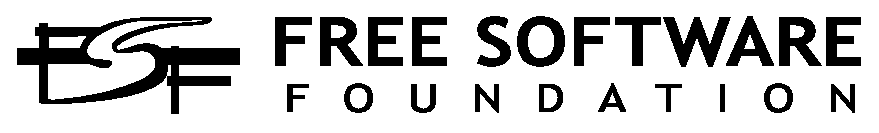
\includegraphics{fsf-logo.eps}

\vspace{0.3in}

{\Huge\bf Qu'est-ce que le logiciel libre?}

\end{center}

\begin{wrapfigure}[15]{l}{2.0in}
 \begin{center}
   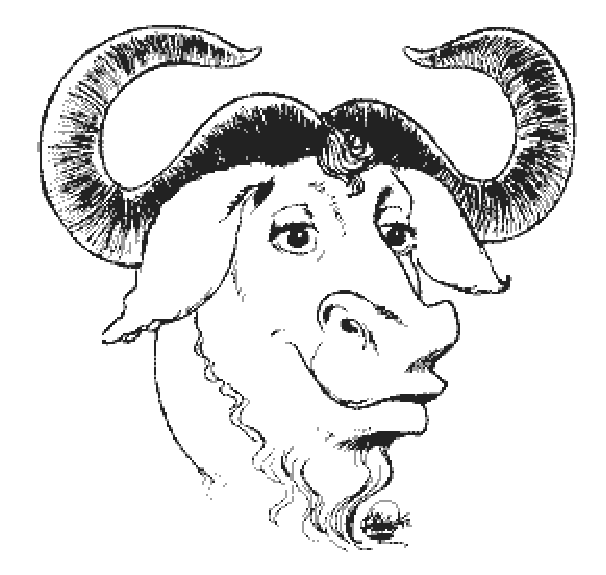
\includegraphics[width=2in]{gnu-head.eps}
 \end{center}
\end{wrapfigure}

Un logiciel libre, c'est un logiciel qui respecte nos libertés. Utiliser un
logiciel libre, c'est faire le choix politique et éthique d'affirmer ses
droits: d'apprendre et de partager ce que l'on apprend avec les autres.

%%Free software is software that respects our freedom. To use free software is to
%%make a political and ethical choice asserting our rights to learn and to share
%%what we learn with others.

Habituellement, les logiciels que nous achetons restreignent nos droits, car ce
n'est pas la propriété du logiciel que nous achetons, mais bien une licence
d'utilisation. Cette licence nous contraint par plusieurs règles, en petits
caractères, stipulant ce que nous pouvons et ne pouvons pas faire.

%%Usually software we buy denies us these rights, because we don't actually buy
%%ownership of the software. Instead, we receive a license to use the software,
%%and this license binds us with many fine-print rules about what we can and
%%can't do.

En copiant le logiciel pour le donner à un ami, en essayant d'apprendre le
fonctionnement d'un programme, en l'installant sur plus d'une de nos propres
machines, dans notre propre maison, nous sommes passibles d'une amende ou d'une
peine de prison. Voilà ce qui se trouve dans les petits caractères.

%%If we make a copy and give it to a friend, if we try to figure out how the
%%program works, if we put a copy on more than one of our own computers in our
%%own home, we could if caught be fined or put in jail. That's what's in the fine
%%print.

Que se passerait-il, s'il y avait un groupe mondial de programmeurs éthiques et
talentueux dévoués à l'idée d'écrire et de partager des logiciels avec tous
ceux qui sont d'accord de les partager sous les mêmes conditions? Que se
passerait-il, si tout le monde pouvait faire partie et bénéficier de cette
communauté, sans pour autant connaitre la programmation? Nous n'aurions plus
peur de nous faire prendre à copier un logiciel pour un ami, car ça ne serait
plus illégal.

%%What if there were a worldwide group of talented ethical programmers
%%voluntarily committed to the idea of writing and sharing software with each
%%other and with anyone else who agreed to share alike? What if anyone could be a
%%part of and benefit from this community even without knowing anything about
%%programming? We wouldn't have to worry about getting caught copying a useful
%%program for our friends---because we wouldn't be doing anything illegal.

\begin{wrapfigure}[15]{r}{1.5in}
 \begin{center}
   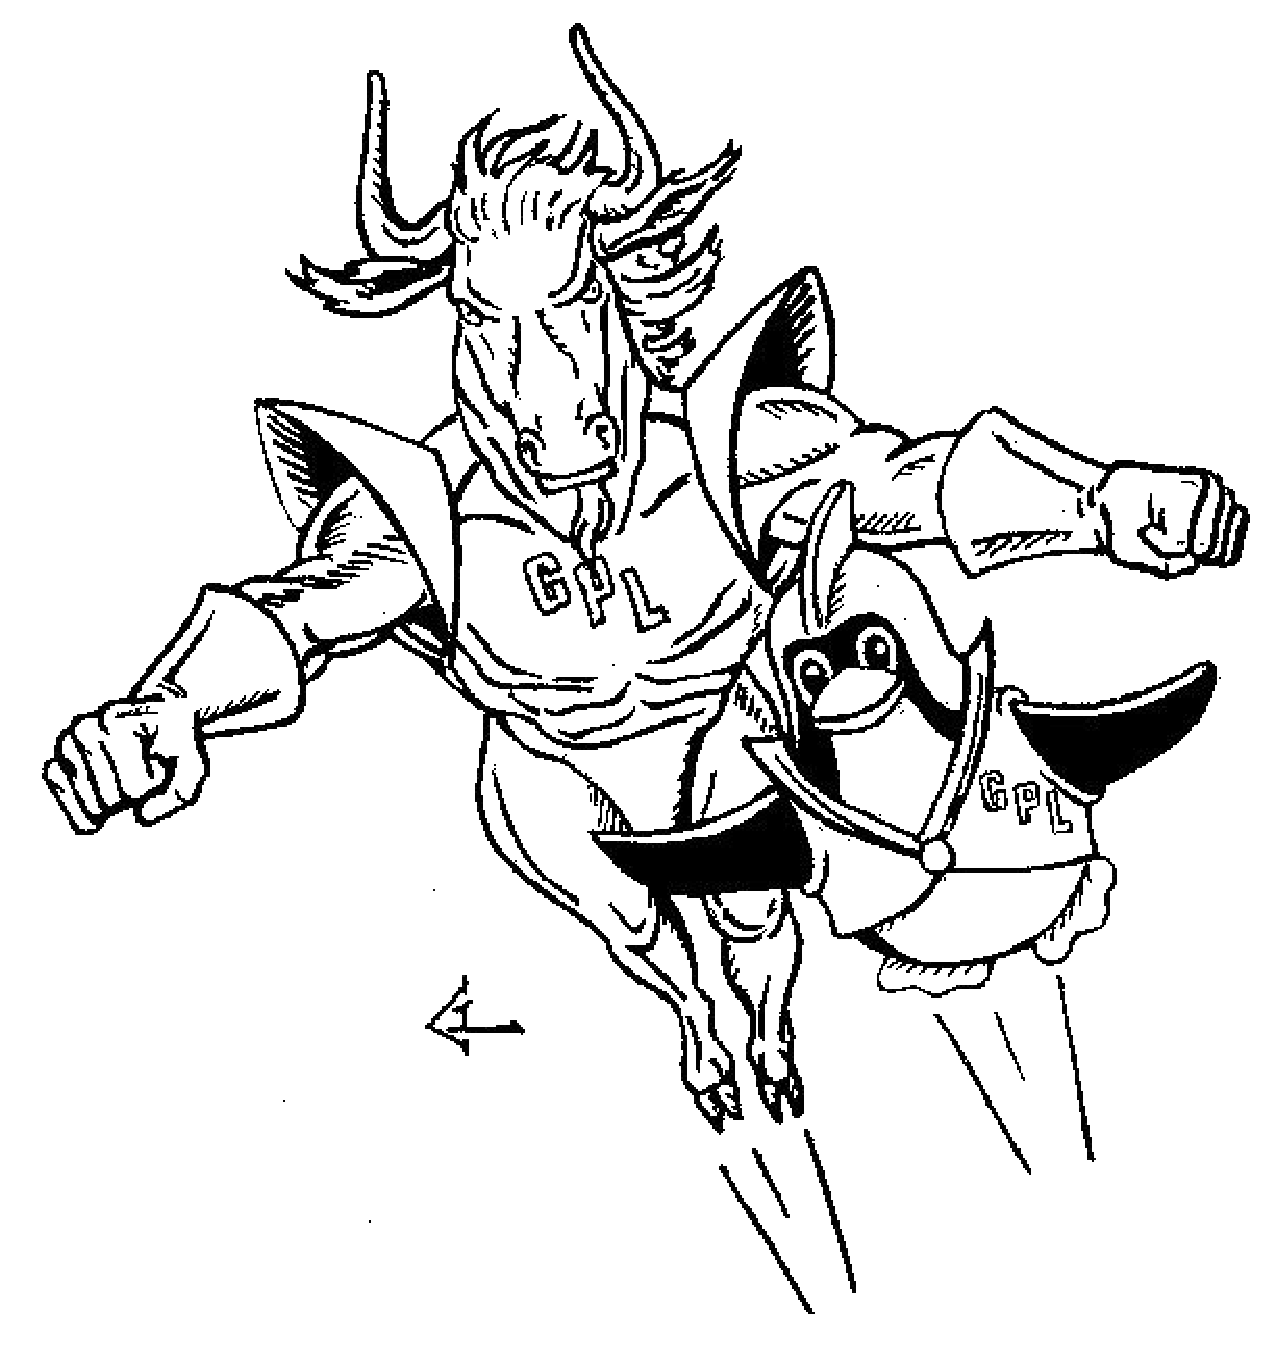
\includegraphics[scale=0.22]{dynamic-duo-bw.eps}
 \end{center}
\end{wrapfigure}

\begin{center}
{\Large\bf Le mouvement du logiciel libre}
\end{center}

En fait, un tel mouvement existe, et vous pouvez en faire partie. Le mouvement
du logiciel libre a débuté avec Richard M. Stallman, en 1984, lorsqu'il a
démarré le projet GNU, qui signifie \guillemotleft GNU's Not
UNIX\guillemotright, afin de fournir un remplacement pour le système
d'opération UNIX, un remplacement qui respecte les libertés de ceux qui
l'utilisent. En 1985, Stallman fonda la Free Software Foundation, une
organisation à but non lucratif qui a pour mission de défendre et d'éduquer au
nom des utilisateurs du monde entier.

%%In fact, such a movement exists, and you can be a part of it. The free software
%%movement was started in 1984 by Richard M. Stallman, when he launched a project
%%called GNU, which stands for ``GNU's Not UNIX'', to provide a replacement for
%%the UNIX operating system---a replacement that would respect the freedoms of
%%those using it. Then in 1985, Stallman started the Free Software Foundation, a
%%nonprofit with the mission of advocating and educating on behalf of computer
%%users around the world.

Aujourd'hui, l'infiltration technologique mondiale diminue constamment le
nombre de personnes qui n'utilisent pas un ordinateur. Faire fonctionner cette
technologie requiert des connaissances. Un savoir accaparé par des personnes,
qui menacent et punissent ceux qui désirent l'obtenir et le partager.
Contrairement à leurs prétentions, ces personnes n'ont pas pour objectif de
préserver ce savoir, mais bien de préserver ce pouvoir pour eux-mêmes au
détriment des libertés des autres.

%%Today the number of people who are not computer users is dwindling all the
%%time, as technology seeps around the globe. It takes knowledge to make this
%%technology work. People who hoard this knowledge, punishing and threatening
%%others who try to obtain and share it, are not doing so in order to preserve
%%it, despite what they may claim. Instead, they are preserving power for
%%themselves at the expense of others' freedom.

\begin{wrapfigure}[10]{l}{2in}
  \vspace{-0.25in}
  \begin{center}
    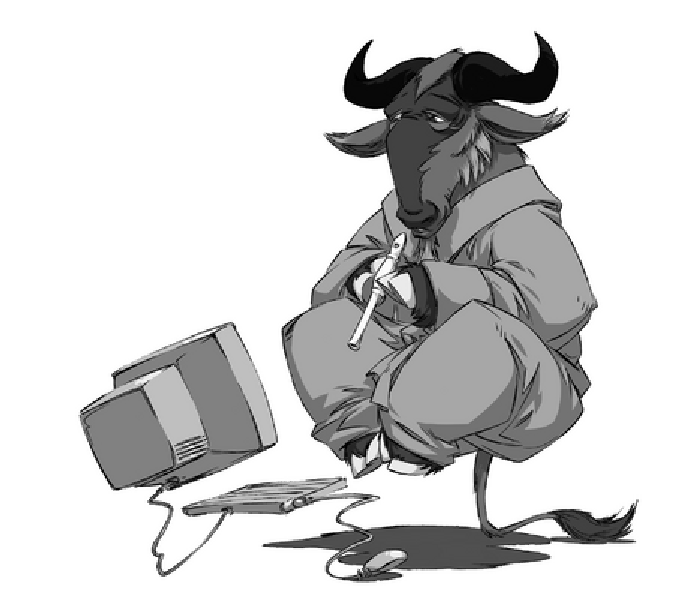
\includegraphics[scale=0.45]{gnu-think-smaller.eps}
  \end{center}
\end{wrapfigure}

Reconnaissant cela, des millions de personnes à travers le monde---incluant des
gouvernements---se sont engagés à utiliser le logiciel libre sur leurs
ordinateurs. Le fait que tant de personnes soient prêtes à prendre cette
décision face à des propositions de plus en plus ``abordable'' de Microsoft,
Apple et d'autres compagnies de logiciels propriétaires prouve que ces
compangies sont dans le tort---nous n'avons pas besoin d'eux ou de leur
permission pour faire du logiciel.

%Recognizing this, millions of people around the world---including entire
%governments---have made the commitment to use only free software on their
%computers. The fact that so many people are willing to make and stand by this
%decision in the face of cheaper and cheaper ``deals'' from Microsoft, Apple and
%other proprietary software companies proves these companies wrong---we don't
%need them or their fine print to make software.

Nous pouvons le faire nous même. Nous le faisons déjà nous même.

%We can do it ourselves. We are doing it ourselves.

\begin{center}
%{\Large\bf How Does It Work? Copyleft!}
{\Large\bf Comment ça marche? Copyleft!}
\end{center}

Puisque les lois sur la propriété intellectuelle couvrant le logiciel sont
souvent utilisées pour faire disparaître nos libertés, Stallman et la FSF ont
développé un document légal spécifique appelé le GNU General Public
License(GPL) afin de nous protéger. Au lieu de restreindre ce que nous pouvons
faire avec le logiciel, la GPL nous encourage à apprendre et à partager. C'est
pourquoi l'on appele cette license ``copyleft''. Des milliers de personnes et
d'entreprises---des amateurs aux grosses entreprises comme IBM et
Novell---contribuent et distribuent le logiciel libre en utilisant la GPL.

%Because the copyright laws covering software are often used to take away our
%freedoms, Stallman and the FSF developed a specific legal document called the
%GNU General Public License (GPL) to protect them. Instead of restricting what
%we can do with software the GPL encourages us to learn and share, so it is
%called a ``copyleft'' license. Thousands of people and businesses---from
%hobbyists to big companies like IBM and Novell---are now authoring and
%distributing free software using the GPL.

Chaque logiciel à utiliser est un choix politique pour nous tous, pas seulement
pour ceux qui le programment et le vendent. Nous pouvons perdre nos libertés
simplement en cliquant {\tt OK} dans une fenêtre Microsoft et Macintosh après
avoir lu attentivement les trentes pages de restrictions, ou nous pouvons
cliquer sur {\tt CANCEL}, et voir s'il existe un logiciel libre qui répond à
nos besoins.

%But which software to use is a political choice for all of us, not just the
%people who program and sell it. We can click our freedoms away by signaling
%{\tt OK} in the Microsoft or Macintosh window after squinting through their
%thirty pages of restrictions, or we can click {\tt CANCEL}, and see instead if
%there is a piece of free software that does what we need.

Nous devrions cliquer sur {\tt CANCEL} lorsque nous le pouvons puisque c'est le
choix le plus éthique. Cela veut dire que nous allons devoir apprendre un
nouveau programme, et il se peut que ce programme libre pourrait ne pas
fonctionner. Le choix éthique n'est pas toujours le choix facile.

%We should click {\tt CANCEL} when we can because that's the more ethical choice.
%This means we'll have to learn a new program, and sometimes the free program
%might not work as well. The ethical choice is not always the easy choice.

\begin{center}
{\Large\bf Impliquez-vous}
\end{center}

Vous pouvez commencer par l'engagement de considérer des alternatives libres à
vos logiciels. Pour se faire, le \textit{Free Software Directory}
(\url{http://directory.fsf.org}) énumère plus de 5000 logiciels.

%You can start by making a commitment to look for free software alternatives.
%The Free Software Directory (\url{http://directory.fsf.org}) lists over 5,000 free
%programs.

Il y a plusieurs façons pour les personnes avec et sans compétences en
programmation d'aider le mouvement du logiciel libre à continuer de réussir.
Consultez le site de la \textit{Free Software Foundation}
(\url{http://www.fsf.org}) et du projet GNU (\url{http://www.gnu.org}) pour
plus d'information.

Et bien sur, faites des copies de cette information et partagez avec les
autres.

%There are many other ways for people with and without programming skills to
%help the free software movement continue to succeed. Please see the websites of
%the Free Software Foundation (\url{http://www.fsf.org}) and the GNU project,
%(\url{http://www.gnu.org}) to find out how.

%And of course, please make copies of this information and share it with
%others!

\vspace{0.3in}

{\small

\noindent Copyright \copyright\/ 2000, 2001, 2005, 2006 Free Software Foundation, Inc., 51
Franklin Street, 5th Floor, Boston, MA 02110, USA.

Verbatim la copie et la distribution de ce document est permise sur tout support,
que cette notice soit préservée.

%Verbatim copying and distribution of this entire article is permitted
%in any medium, provided this notice is preserved.
}

\end{document}
